\documentclass[12pt]{article}
%\usepackage{snapshot}  % Creates .dep file showing dependencies
\usepackage[a4paper, margin=0.5in]{geometry}

\usepackage{anyfontsize}
\usepackage{xcolor}
\usepackage{graphicx}
\usepackage{setspace}
\usepackage{hyperref}
\usepackage{booktabs}
\usepackage[backend=biber]{biblatex}
\usepackage{float}
\usepackage{siunitx}
\usepackage{svg}
\usepackage{xepersian}
\usepackage{algorithm2e}
\usepackage{caption}
\usepackage{amssymb}
\usepackage{amsmath}
\usepackage{enumitem}
\usepackage{bigints}
\hypersetup{colorlinks,urlcolor=blue}
%\settextfont[Scale=1.1]{Far.Mitra}

\settextfont[Scale=1.0, Size=14pt]{B Nazanin}
\defpersianfont\persiantitlefont[Scale=1.0, Size=18pt]{B Titr}
\setlatintextfont[Scale=1.0, Size=12pt]{Times New Roman}
\deflatinfont\englishtitlefont[Scale=1.0, Size=16pt]{Times New Roman Bold}

\usepackage[backend=biber]{biblatex}
\addbibresource{references.bib}


\def\labelitemi{$\diamond$}
\def\labelitemii{$\ast$}
\setcounter{secnumdepth}{0}  % Depth 0 = no section numbering

\begin{document}
	\linespread{3}
	\setstretch{1.5}
	
	% --- HEADER ROW ---
	\begin{minipage}[t]{0.7\textwidth}
		\huge\textcolor{teal!70!black}{\title\textbf{{استنباط آماری}}}
	\end{minipage}
	\hfil
	\begin{minipage}[t]{0.15\textwidth}
		\centering
		
\includegraphics[width=0.9\linewidth]{pics/logo.png}\\[6pt]
		{\small پاییز ۱۴۰۴}
	\end{minipage}
	
	
	
	{
		
		\Large{تمرین سوم}
		
		\large مرتضی ملکی‌نژاد شوشتری - ۸۱۰۱۰۴۲۵۶
		
		
	}
	
	\vspace{1.2cm}
	
	
	
	\vspace{0.3cm}
	\hrule
	\vspace{0.6cm}
%	\tableofcontents
	\section*{سوال ۱}
\subsection{1}
فرض صفر این است که 
$
\mu_A \geq \mu_B
$
و فرض جایگزین این است که 
$
\mu_A < \mu_B
$.

این یک تست 
\lr{one tail}
است و برای بررسی آن باید 
یک 
\lr{two sampled t test}
انجام شود.
\subsection{۲}
باید 
\lr{pooled variance}
حساب شود:
\begin{latin}
	$
	s_p^2  = \cfrac{(n_A - 1)s_A^2 + (n_B - 1)s_B^2}{n_A + n_B - 2}
	= 
	\cfrac{9 * 16 + 99 * 625 }{108} \approx 574.25 
	\Rightarrow s_p = \sqrt{574.25} \approx 23.96 
	$
\end{latin}
حال با استفاده از 
\lr{pooled variance}
می‌توان 
\lr{test statistic}
را حساب کرد و سپس آن را با یک توزیع 
\lr{t}
با 
$n_A + n_B - 2$
درجه آزادی
مقایسه کرد:
\begin{latin}
	$
	t = \cfrac{\bar{x}_A - \bar{x}_B}{s_p \sqrt{\cfrac{1}{n_A} + \cfrac{1}{n_B}}}
	\approx \cfrac{-6}{7.947} \approx -0.755
	\\
	critical\ value: t_{0.05,108} \approx -1.659 \Rightarrow Reject\ if\ h_0 < -1.659
	\\
	-0.755 > -1.659 \Rightarrow h_0\ is\ not\ rejected
	$
\end{latin}
پس یعنی فرض صفر رد نمی‌شود.

\subsection{۳}
داریم:
\begin{latin}
	$
	t = \cfrac{\bar{x}_A - \bar{x}_B}{\sqrt{\cfrac{s_A^2}{n_1} + \cfrac{s_B^2}{n_2}}}
	= \cfrac{-6}{\sqrt{1.6 + 6.25}} \approx -2.142
	\\\\
dof = 10 - 9 = 9 \Rightarrow Critical\ value = t_{0.05, 9} \approx -1.83
	$
\end{latin}
چون مقدار 
\lr{test statistic }
از مقدار 
\lr{critical value}
کمتر نیست فرض صفر رد نمی‌شود.
\subsection{۴}
در اینجا یکی شد. در حالت کلی تست \lr{unpooled} چون واریانسی بیشتر از 
\lr{pooled variance}
نیاز دارد،‌ معمولا 
\lr{critical region}
کوچکتری دارد و اگر تست 
\lr{pooled}
رد نشود، احتمال رد شدن این تست کمتر است.
\subsection{۵}
با استفاده از 
\lr{welch t test}
داریم
\cite{welchs_t_test}
:
\begin{latin}
	$
		dof = \cfrac{(\cfrac{s_A^2}{n_1} + \cfrac{s_B^2}{n_2})^2}{\cfrac{(\cfrac{s_A^2}{n_1})^2}{n_1 - 1} + \cfrac{(\cfrac{s_B^2}{n_2})^2}{n_2 - 1}}
		= \cfrac{(1.6 + 6.25)^2}{\cfrac{2.56}{9} + \cfrac{39.0625}{99}}
		\approx 179.10
		t_{0.05, 179.10} = -1.653
	$
\end{latin}
یعنی باز هم تست فرض صفر را رد نمی‌کند.
	\section{سوال ۲}
	\lr{\subsection{1. Modeling and parameter of interest}}
\lr{\subsubsection{a}}
\begin{latin}
	$
	x = after - before
	$
\end{latin}	
\lr{\subsubsection{b}}
پارامتری از جمعیت که این آماره تخمین می‌زند تفاوت مقدار لگاریتم‌ها است. یعنی داریم:
\begin{latin}
	$
	x = log(after) - log(before) = log (\cfrac{after}{before}) \Rightarrow exp(x) = \cfrac{after}{before} 
	$
\end{latin}
پس یعنی می‌توان با این آماره، نسبت گلوکز قبل و بعد مصرف اندازه گرفت.

در تست‌ها چیزی که اندازه گرفته می‌شود، میانگین این پارامتر است.
\lr{\subsection{2. Hypothesis formulation}}
\lr{\subsubsection{a}}
فرض صفر انتظار دارد که دارو مقدار گلوکز را کاهش ندهد، پس یعنی نسبت میزان گلوکز بعد از مصرف به قبل از مصرف از یک بیشتر باشد پس یعنی مقدار
$x$
از صفر بیشتر باشد:
\begin{latin}
	$
	\\
	H_0: \bar{x} \geq 0 \\
	H_1: \bar{x} < 0
	$
\end{latin}
\lr{\subsubsection{b}}
همانطور که بیان شد، اگر دارو تاثیری در کاهش مقدار گلوکز نداشته باشد، داریم:
\begin{latin}
	$
	after \geq before \Rightarrow \cfrac{after}{before} \geq 1 
	\Rightarrow log(\cfrac{after}{before}) \geq 0
	\Rightarrow log(after) - log(before) \geq 0
	$
\end{latin}
\lr{\subsubsection{c}}
در صورت سوال بیان شد که پس از گرفتن لگاریتم، خاصیت نویز‌ها بصورت جمع در می‌آید، پس یعنی انگار
$x$
حاصل جمع تعدادی متغیر تصادفی است. اگر تعداد این متغیرها زیاد باشد (که درموضوعی مثل میزان قندخون، عوامل زیادی دخیل هستند و این فرض بعید نیست.) طبق قضیه حد مرکزی، توزیع 
\lr{x}
از یک توزیع نرمال تبعیت می‌کند، پس 
\lr{t test}
مناسب است. از آنجایی که تعداد نمونه‌ها به نسبت کم است باید از توزیع 
\lr{t}
استفاده کرد. و میانگین مقادیر 
\lr{x}
را چک کرد.
\lr{\subsection{3. Inference}}
\lr{\subsubsection{a}}
\begin{latin}
		$
		\\
	\bar{x} = \cfrac{1}{15} \sum (After - Before) = 0.06
	\qquad 
	s \approx 0.046
	\\
	statistic = \cfrac{\bar{x} - \mu_0}{\cfrac{s}{\sqrt{n}}} \approx -5.09
	$
\end{latin}
\lr{\subsubsection{b}}
\begin{latin}
	$
	dof = n - 1 = 14 \quad
	p_{value} = P(t_{14} < t) \approx 0.00008
	$
\end{latin}
همانطور که حساب شد،  مقدار 
\lr{p value}
با اختلاف از مقدار 
$\alpha$
کمتر است یعنی تست فرض صفر را رد می‌کند.
\lr{\subsection{4. Interval estimation}}
\lr{\subsubsection{a}}
\begin{latin}
	$
	\bar{x} = -0.06 \quad
	s = 004 \qquad CI = [\bar{x} - t_{14,0.95} * \cfrac{s}{\sqrt{n}}, \bar{x} + t_{14,0.95} * \cfrac{s}{\sqrt{n}}]
	\Rightarrow 
	CI_{0.95} \approx [-0.08, -0.03]
	$
\end{latin}
\lr{\subsubsection{b}}
با به توان رساندن داریم:
\begin{latin}
	$
	exp \Rightarrow e^{CI} \approx [0.92, 0.96]
	$
	
\end{latin}
یعنی به احتمال ۹۵ درصد، میانگین کاهش گلوکز چیزی حدود چهار تا هشت درصد است.
\lr{\subsection{5. Diagnostic reasoning}}
\lr{\subsubsection{a}}
با این‌کار، داده‌ها از فضای پیوسته به فضای گسسته می‌آیند و نمی‌توان درباره پراکندگی و یا مقدار تاثیر صحبتی کرد. همچنین بین داده‌ای که تنها ۰.۰۱ کمتر شده و داده‌ای که ۰.۰۹ کمتر شده فرقی نیست. استفاده از همچنین چیزی در شرایطی که داده‌های بهتری داریم منطقی نیست. 

در عمل اینکار شبیه به 
\lr{sign test}
است و در جاهایی که توزیع و مقادیر معلوم هستند، تست‌های پارامتریک از این تست بهتر هستند.

\lr{\subsubsection{b}}
پراکندگی و میزان تاثیر دارو از دست می‌روند و در کیفیت تست به اینصورت اثر دارند که تست حاصل شده، از
\lr{power}
کمتری برخوردار خواهد بود. همچنین دیگر نمی‌توان درباره میزان تاثیر دارو صحبتی کرد.

\section{سوال ۳}
\subsection{۱}
این یک 
\lr{matched test}
است. در هر گروه باید میزان بهبود را حساب کرد و سپس میانگین و واریانس نمونه‌ای حساب شود و تست روی آن انجام شود. 
\begin{latin}
	$
	diff = drug\ change - placebo\ change \qquad
	t = \cfrac{\bar{diff}}{\cfrac{\sigma}{\sqrt{n}}}
	$
\end{latin}
با انجام محاسبات، مقدار \lr{p value} در هرگروه بدست می‌آید:
\begin{table}[H]
	\centering
	\caption{مقدار \lr{p value} در هر دسته}
	\begin{latin}
		\label{tab:q3_table}
		\begin{tabular}{| l l  |}
			\toprule
			\textbf{Warden} &  \textbf{P Value} \\
			A & 0.11 \\
			B & 0.22 \\
			\bottomrule
		\end{tabular}
	\end{latin}
\end{table}
یعنی در هر دو گروه، تست \lr{t} با 
\lr{confidence level}
برابر با ۰.۹۵ نمی‌تواند فرض صفر را رد کند.

\section{سوال ۴}
با توجه به اینکه در اینجا مسئله تعداد اعضای هر دسته است می‌توان از 
\lr{chi squared goodness of fit}
استفاده کرد. داریم:
\begin{latin}
	$
    \sum\limits_{i = 1}^k	\cfrac{O_i - E_i}{E_i} \sim \chi^2_{k - 1}
	$
\end{latin}
پس در اینجا داریم:
\begin{latin}
	$
	\sum\limits_{i = 1}^k	\cfrac{(O_i - E_i)^2}{E_i} 
	=
	\sum\limits_{i = 1}^k	\cfrac{(N_i - 80)^2}{80} 
	=
	\sum\limits_{i = 1}^k	\cfrac{N_i^2 - 160 N_i + 6400}{80}
	=
	\sum\limits_{i = 1}^k	\cfrac{N_i^2}{80} + (80 - 2N_i)
	=
	\sum\limits_{i = 1}^k	\cfrac{N_i^2}{80} + 400 - 2 * 400
	=
	\sum\limits_{i = 1}^k	\cfrac{N_i^2}{80} - 400
	\sim \chi^2_4
	$
\end{latin}
از آنجایی که تست با 
\lr{confidence level}
برابر با ۰.۰۱ است، برای 
\lr{critical value}
باید مقدار 
\lr{ppf}
مربوط به 
$\chi_{0.99, 4}$
را حساب کرد که تقریبا برابر است با
$13.277$
پس داریم:
\begin{latin}
	$
	\sum\limits_{i = 1}^k	\cfrac{N_i^2}{80} - 400 > 13.277
	\Rightarrow
	\sum\limits_{i = 1}^k	\cfrac{N_i^2}{80} > 413.277
	\Rightarrow
	\sum\limits_{i = 1}^k	N_i^2 > 33061.6
	$
\end{latin}
\section{سوال ۶}
\subsection{۱}
تست از نوع 
\lr{one sample}
و 
\lr{two tail }
است.
مقدار 
\lr{significance level}
برابر است با 
$P(reject\ H_0 | H_0 )$
یعنی :

\begin{latin}
	$
	P(X < 60 | p = 0.7) + P(X > 80 | p = 0.7)
	$
\end{latin}
با استفاده از فرمول 
\lr{PMF}
توزیع دوجمله‌ای داریم:
\begin{latin}
	$
	P(X = x) = C(n, x) (p^x) (1 - p)^{n - x} 
	= 
	C(100, x) * 0.7^{x} * 0.3^{100 - }
	$
\end{latin}
با محاسبه مقدار 
	$
P(X < 60 | p = 0.7) + P(X > 80 | p = 0.7)
$
به این می‌رسیم:
$
P(X < 60 | p = 0.7) + P(X > 80 | p = 0.7) \approx 0.021
$
یعنی مقدار 
$\alpha$
تقریبا برابر 
$0.021$
است.
\subsection{۲}
{
\centering
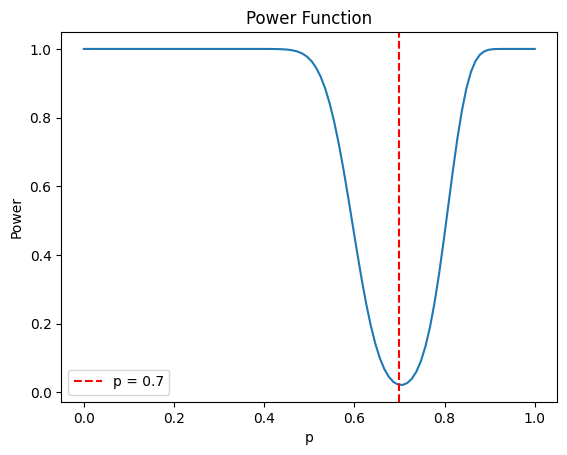
\includegraphics[width=0.8\textwidth]{pics/q6.png}
\captionof{figure}{مقدار \lr{power} به ازای مقادیر مختلف \lr{p}}
}
\subsection{۳}
\lr{\subsubsection{a}}

\begin{latin}
	$
	Critical\ value = P(|X - 70| \geq 2 | p = 0.7) = 1 - P(X = 69 ) - P(X = 70) - P(X = 71) \approx 0.74
	$
\end{latin}
اگر مقدار 
$\alpha$
از این مقدار بیشتر باشد فرض صفر رد می‌شود ولی در هیچ تست منطقی‌ای مقدار 
$\alpha$
اینقدر زیاد نیست.
\lr{\subsection{b}}
داریم:
\begin{latin}
	$
	\mu = np = 70 \quad 
	\sigma = \sqrt{n p (1 - p)} \approx 4.58
	\Rightarrow
	z = \cfrac{S + correction - \mu}{\sigma}
	\Rightarrow Z_{correction} = \cfrac{3}{4.58 } \approx 0.55 \quad 
	z_{without\ correction} = \cfrac{2.5}{4.58 } \approx 0.66
	$
\end{latin}
حال برای محاسبه 
\lr{critical value}
داریم:
\begin{latin}
	$
	P(|Z| > z_{crrection}) \approx 2 * 0.29 = 0.58 
	\\
	P(|Z| > z_{without\ crrection}) \approx 2 * 0.29 = 0.5
	\\
	$
\end{latin}
\section{سوال ۷}
\subsection{۱}
	دراینجا باید از آزمون 
	\lr{chi squared goodness of fit}
	استفاده کرد. 
	
	برای محاسبه مقدار \lr{expect} می‌توان از  \lr{pdf} توزیع دوجمله‌ای استفاده کرد. 
	طبق داده‌های سوال داریم:
	\begin{table}[H]
		\centering
		\caption{مقدار \lr{p value} در هر دسته}
		\begin{latin}
			\label{tab:q7_table}
			\begin{tabular}{| l l l  |}
				\toprule
				\textbf{Number of boys} &  \textbf{Expect} & \textbf{Ovserve} \\
				0 & 16 & 26 \\
				1 &48 & 32 \\
				2 & 48 & 40 \\
				3 & 16 & 30 \\
				\bottomrule
			\end{tabular}
		\end{latin}
	\end{table}
	سوال عملا مقدار 
	\lr{p value}
	را می‌خواهد پس داریم:
	\begin{latin}
		$
		\sum_i=0^3 \cfrac{(O_i - E_i)^2}{E_i} \approx 25.16
		\\
		p\_value = 1 - cdf_3(25.16) \approx 1.42e-5
		$
	\end{latin}
	پس یعنی به‌ازای 
	$\alpha < 1.42e-5$
	تست فرض صفر را رد نمی‌کند. و به‌ازای سایر مقادیر فرض صفر رد می‌شود.
	\subsection{۲}
	دراینجا باید از 
	\lr{ump}
	استفاده کرد و شبیه قسمت قبل عمل کرد، صررفا بجای استفاده از یک 
	\lr{p}
	مشخص 
	از 
	\lr{p}
	مربوط به 
	\lr{maximum likelihood}
	استفاده کرد:
	\begin{latin}
		$
		P(x) = C(3, x) * (p^x) * (1 - p)^{3 - x}
		\Rightarrow 
		P_{total} = \prod\limits_{i = 0}^3 C(3, i) *  (p^i) * (1 - p)^{3 - i}
		= 
		 1 * 3 * 3 * 1 * p^6 * (1 - p)^6
		 = 
		 9 * (p - p^2)^6
		$
	\end{latin}
	اگر مقدار قدرمطلق 
	$p - p^2$
	بیشینه باشد، مقدار 
	\lr{likelihood}
	بیشینه می‌شود (به شرط اینکه $0<p<1$). پس یعنی در 	$p=0.5$ تابع بیشینه می‌شود. پس یعنی عملا نتایج قسمت قبل که با 
	$p=0.5$ 
	حساب شدند،‌همان نتایج مربوط به 
	\lr{UMP}
	هستند. و در همان 
		$\alpha < 1.42e-5$
		فرض صفر رد نمی‌شود.  و به‌ازای سایر مقادیر فرض صفر رد می‌شود.
		\section{سوال ۱۰}
		\subsection{۱}
		\lr{\subsubsection{a}}
		این یک تست 
		\lr{one sampled} 
		برای میانه است و می‌توان از آزمونی مثل 
		\lr{sign test}
		برای آن استفاده کرد.
		\begin{latin}
			$
			H_0: \text{median} \geq 120
			\\
			H_1: \text{median} < 120
			$
		\end{latin}
	\lr{\subsection{b}}
	داریم:
	\begin{latin}
		$
		data - 120 = [5, -10, 10, -2, 20, 0, -15, 15, 2, -1, 25, 30, -5, 8, 1, 18, -8, 0] 
		\Rightarrow t = \text{number of negatives}  = 4 \quad n = 16
		$
	\end{latin}
	برای مقادیری که روی ۱۲۰ هستند،‌ آن‌ها را از تست خارج می‌کنیم و تست را با 
	$n^*=16$
	ادامه می‌دهیم.
	\subsection{۲}
	\lr{\subsubsection{a}}
	برای محاسبه 
	\lr{p value}
	با استفاده از توزیع دوجمله‌ای داریم:
	\begin{latin}
		$
		P(x) = C(16, x)(0.5)^{16}
		\Rightarrow
		P(x \leq 6) = 
		\cfrac{1}{2^{16}} \sum\limits_{i = 0}^6 C(16, i) 
		= \cfrac{14893}{2^{16}} \approx 0.2272
		$
	\end{latin}
	\lr{\subsubsection{b}}
	از آنجایی که 
	\lr{p value}
	از 
	\lr{significance level}
	بزرگ‌تر است، تست فرض صفر را رد نمی‌کند.
	\subsection{۳}
	\lr{\subsubsection{a}}
	داریم:
	\begin{latin}
		$
		\mu = n * p = 16 * 0.5 = 8
		\quad 
		\sigma^2 = n * p * (1 - p) = \cfrac{n}{4} = 4 \Rightarrow \sigma = 2
		z = \cfrac{t + \text{continuity correction } - \mu}{\sigma} = \cfrac{-1.5}{2} = -0.75
		$
	\end{latin}
	\lr{\subsubsection{b}}
	با مراجعه به جدول توزیع نرمال استاندارد داریم 
	$CDF_Z(-0.75) \approx 0.2266$
	که تقریبا با جواب مرحله قبل برابر است و تست همچنان نمی‌تواند فرض صفر را رد کند.
\section{مراجع}
\begin{latin}
	\printbibliography
\end{latin}

	
\end{document}